\label{sec:eval}
\vspace{-2mm}

In all of our experiments we use the same training settings used in~\cite{Kingma2014}; that is,  
we use Adagrad for optimization with minibatches of 100  with a learning rate of 0.01
and a weight decay corresponding to a prior of $\mathcal{N}(0,1)$.
We initialize weights in our network using the heuristic of ~\cite{glorot2010understanding}.
However for the pose recognition modules in the ST-VAE model, we have found it useful to
specifically initialize biases so that poses are initially close to the identity transformation (see~\cite{jaderberg2015spatial}).

We use vanilla VAE models  as a baseline model against first the (single image layer) ST-VAE
model, then the more general CST-VAE model.  In all of our comparison we fix the training time for all models.
We experiment with between 20 and 50  dimensions for the latent content variables $z^C$
and always use 6 dimensions for pose variables $z^T$.
We parameterize content encoders and decoders
by using a two layer fully connected MLP with 256 dimensional
hidden layers and ReLU nonlinearities.
For pose decoders and encoders we also use two layer fully connected MLPs, but 
using 32 dimensional hidden layers and Tanh nonlinearities.
%\footnote{
%
%We have found this choice of Tanh vs. ReLU makes a significant
%difference in practice.
%\kevin{Why?}
%}
Finally for spatial transformer modules, we always resample onto a grid that is the same size as the original
image.


%\Jon{For binary images, it is common to have a sigmoid at the end of the VAE decoder.
%However we have found that it is often more numerically stable in these situations to first apple the spatial transformation, then
%to apply the sigmoid after the transformation.
%}

\begin{figure}[t]
\begin{center}
\subfigure[]{
\raisebox{2mm}{
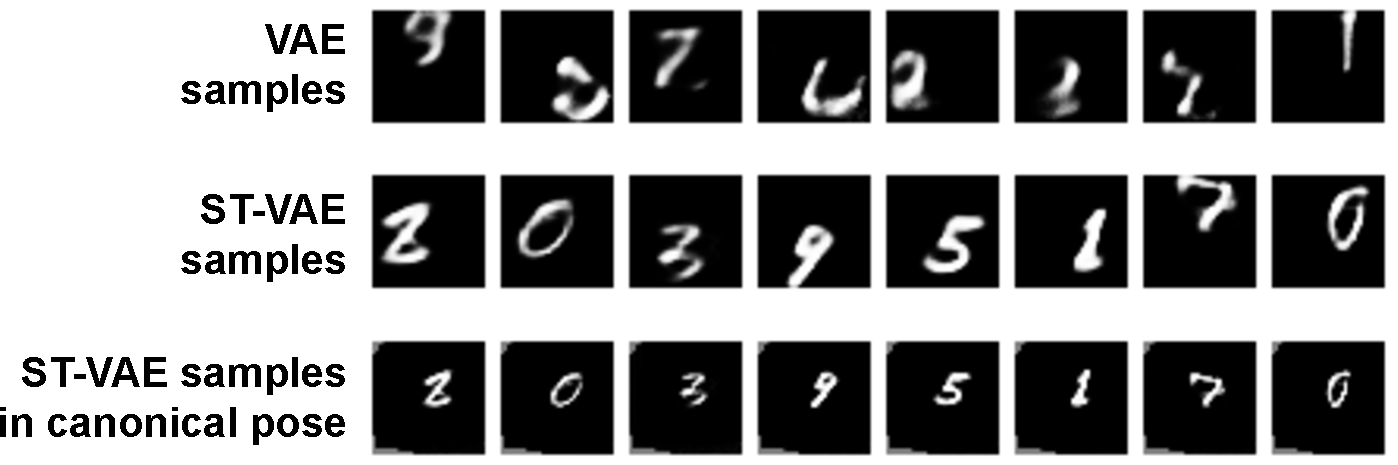
\includegraphics[width=0.48\linewidth]{figs/vae_stvae_samples.pdf}
\label{fig:vae_stvae_samples}
}
}
\,
\subfigure[]{
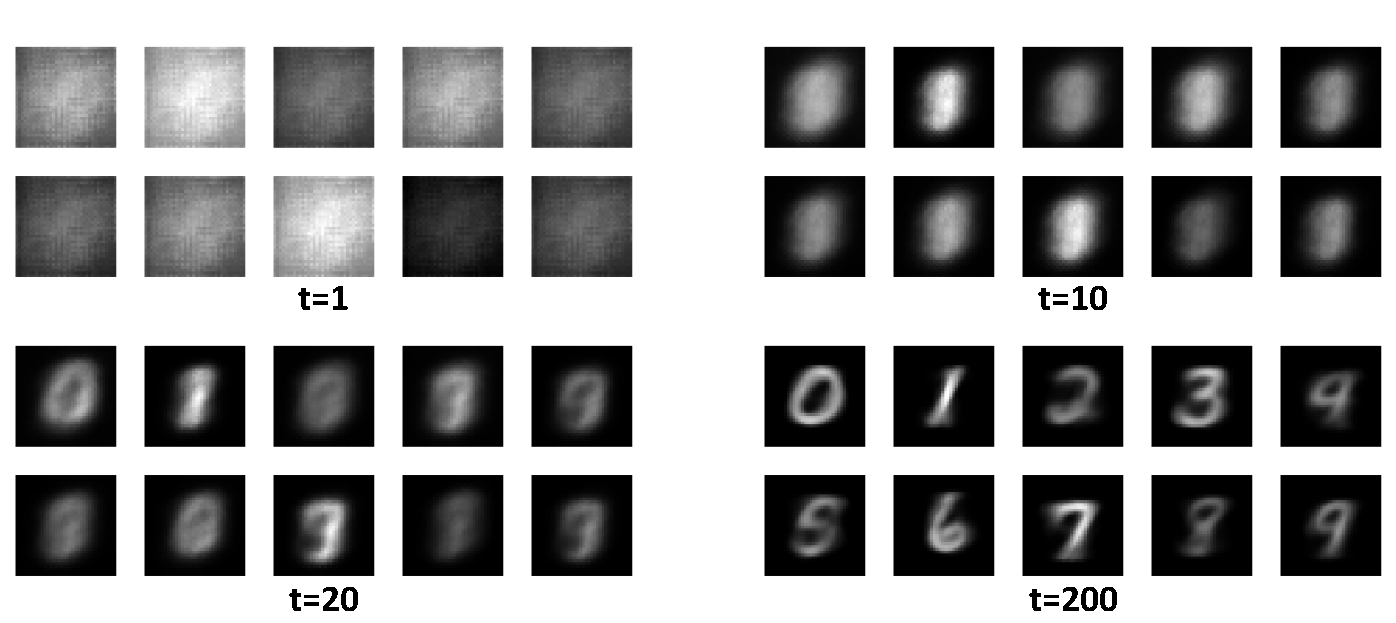
\includegraphics[width=0.45\linewidth]{figs/stvae_averageddigits.pdf}
\label{fig:stvae_averageddigits}
}\vspace{-5mm}
\end{center}
 \caption{\footnotesize
 \subref{fig:vae_stvae_samples} Comparison of samples from the VAE and ST-VAE generative models.  
 For the ST-VAE model, we show both the sample in its canonical pose and the final generated image.
  \subref{fig:stvae_averageddigits}  Averaged images from each MNIST class as learning progresses ---
  we typically see pose variables converge very quickly.
 }\vspace{-2mm}
\end{figure}



\begin{figure}[t]
\begin{center}
\subfigure[]{
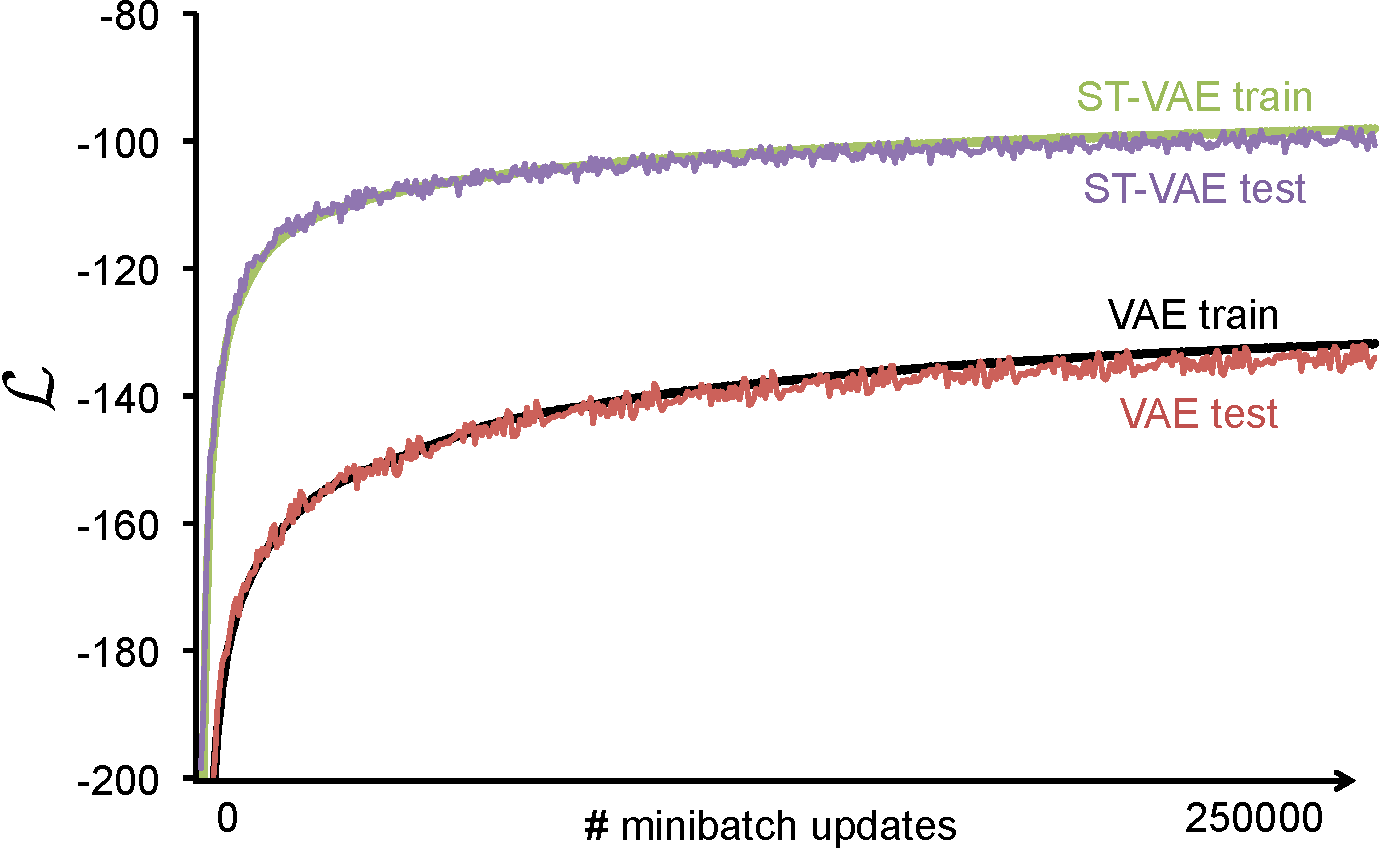
\includegraphics[width=0.30\linewidth]{figs/vae_stvae_learning_curves.pdf}
\label{fig:vae_stvae_learning_curves}
}
\subfigure[]{
\raisebox{12mm}{
\footnotesize
\begin{tabular}{lcc} 
\hline 
%\multicolumn{1}{r|}{Proposals} & \multicolumn{2}{c}{GT} & \multicolumn{2}{c}{multibox} \\
%\multicolumn{1}{r|}{Descriptions} & GEN & GT & GEN & GT \\
 & Train Accuracy & Test Accuracy \\
\hline 
\multicolumn{3}{l}{On translated (36x36) MNIST} \\
\hline
VAE + supervised & 0.771 & 0.146 \\
ST-VAE + supervised & 0.972 & 0.964  \\
directly supervised & 0.884 & 0.783 \\
Directly supervised with STN & 0.993 & 0.969  \\
\hline 
\multicolumn{3}{l}{On original (28x28) MNIST} \\
\hline 
Directly supervised & 0.999 & 0.96   \\
\hline
\end{tabular}%
}
\label{fig:vae_stvae_classification}
}\vspace{-4mm}
\end{center}
 \caption{\footnotesize
 \subref{fig:vae_stvae_learning_curves} Train and test (per-example) lower bounds on log-likelihood 
for the vanilla VAE and ST-VAE models on the Translated MNIST data;
 \subref{fig:vae_stvae_classification} Classification accuracy obtained by supervised training using latent encodings
 from VAE and ST-VAE models.  More details in text.
 }
\end{figure}
\vspace{-2mm}
\subsection{Evaluating the Spatially transformed Variational Autoencoder alone}\vspace{-2mm}

We first evaluate our ST-VAE (single layer) model alone on the MNIST dataset~\citep{lecun1998gradient}
and a derived dataset, \emph{TranslatedMNIST}, in which we randomly translated each  $28\times 28$ MNIST example
within a $36\times 36$ black image.  In both cases, we binarize the images by thresholding at value 128.
Figure~\ref{fig:vae_stvae_learning_curves} plots train and test log-likelihoods over 250000 gradient steps
comparing the vanilla VAE model against the ST-VAE model, where we see that from the beginning the ST-VAE
model is able to achieve a much better likelihood while not overfitting.  This can also be seen in Figure~\ref{fig:vae_stvae_samples}
which visualizes samples from both generative models.   We see that while the VAE model (top row) manages to 
generate randomly transformed blobs on the image, these blobs typically only look somewhat like digits. 
For the ST-VAE model, we plot both the final samples (middle row) as well as the intermediate canonical images (last row), 
which typically are visually closer to MNIST digits. 

Interestingly, the canonical images tend to be slightly smaller versions
of the digits and our model relies on the Spatial Transformer Networks to scale them up at the end of the generative process.
Though we have performed a careful investigation, reasons for this effect may be a combination of the fact (1) that scaling up the images introduces some blur which accounts for small variations in  nearby pixels and (2) it  is easier to encode smaller digits than larger ones.
 We also observe (Figure~\ref{fig:stvae_averageddigits})
that the pose network when trained on our dataset tends to converge rapidly, bringing digits to a centered canonical pose
within tens of gradient updates. 
Once the digits have been aligned, the content network is able to make better progress.

Finally we evaluate the latent content codes $z^C$ learned by our ST-VAE model 
in digit classification using the standard MNIST train/test split.  For this experiment
we use a simple two layer MLP with 32 hidden units in each layer and
ReLU nonlinearities
applied to the posterior mean of $z^C$ inferred from each image; we
do not use the labels to fine tune the VAE.
Figure~\ref{fig:vae_stvae_classification} summarizes the results of the experiment, where we
compare against three baseline classifiers: (1) an MLP learned on latent codes from the VAE model,
(2) an MLP trained directly on Translated MNIST images (we call this the ``directly supervised classifier''), 
and (3) the approach of~\cite{jaderberg2015spatial} using the same MLP as above trained directly
on images but with a spatial transformer network.
As a point of reference, we also provide the performance of our classifier on the original $28\times 28$ MNIST
dataset.  We see that ST-VAE model is able to learn a latent representation of image content that holds enough information
to be competitive with the ~\cite{jaderberg2015spatial} approach (both of which slightly outperform performance
that can be obtained with this MLP training directly on the original MNIST set).  The approaches that do not account for
pose variation do much worse than ST-VAE on this task and exhibit significant overfitting.

\vspace{-2mm}
\subsection{Evaluating the CST Variational Autoencoder}
\vspace{-2mm}

\begin{figure}[t]
\begin{center}
\subfigure[]{
\raisebox{7mm}{
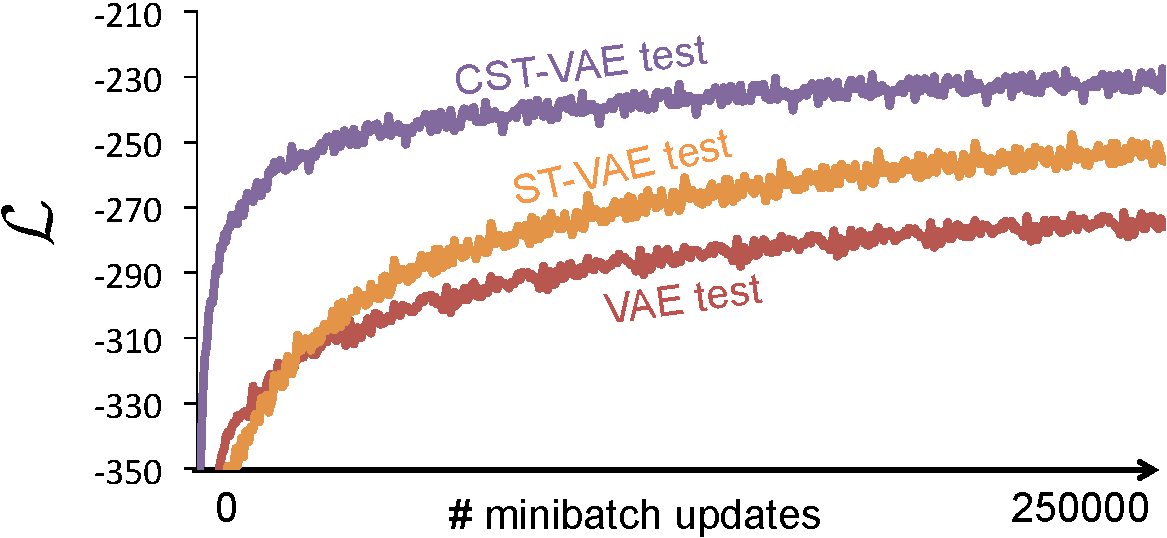
\includegraphics[width=0.35\linewidth]{figs/cstvae_learning_curves2.pdf}
\label{fig:cstvae_learning_curves}
}
}\;
\subfigure[]{
\raisebox{5mm}{
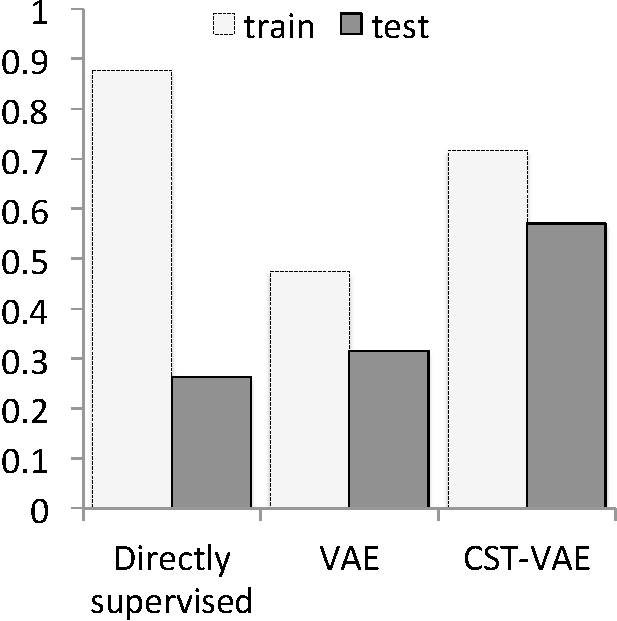
\includegraphics[width=0.2\linewidth]{figs/cstvae_classification.pdf}
\label{fig:cstvae_classification}
}
}\;
\subfigure[]{
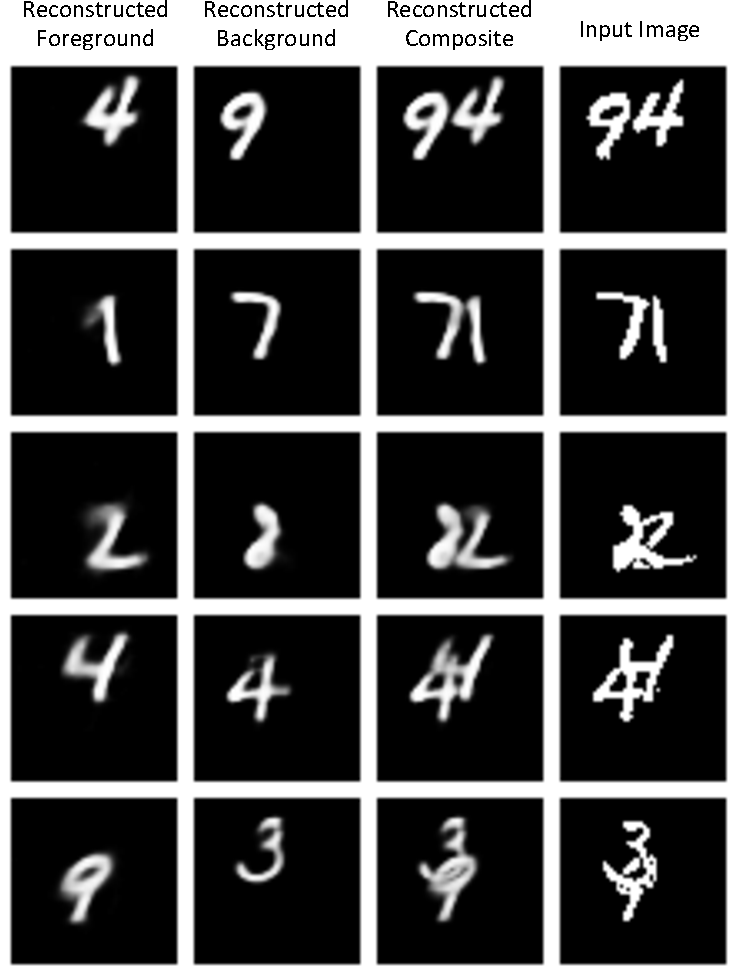
\includegraphics[width=0.35\linewidth]{figs/cstvae_reconstructions.pdf}
\label{fig:cstvae_reconstructions}
}\vspace{-4mm}
\end{center}
 \caption{\footnotesize
 \subref{fig:cstvae_learning_curves} Train and test (per-example) lower bounds on log-likelihood 
for the vanilla VAE and CST-VAE models on the Superimposed MNIST data;
  \subref{fig:cstvae_classification}
 Classification accuracy obtained by supervised training using latent encodings
 from VAE and CST-VAE models on the Supervised MNIST dataset.  More details in text.
 \subref{fig:cstvae_reconstructions}  Images from the Superimposed MNIST dataset with visualizations of
 intermediate variables in the neural network corresponding to first and second layers and the final reconstruction.
 Chance performance on this task is 0.018 (1.8\% accuracy) since we require that the image recover both digits correctly
 within an image.}
\end{figure}



%Dataset
%\begin{itemize}
%\item MNIST superimposed
%\item Can we also get this to work with silhouettes of different grayscale levels?
%\item CIFAR???
%\item Textures
%\end{itemize}

We now show results from the CST-VAE model on a challenging ``Superimposed MNIST'' dataset.
We constructed this dataset
by randomly translating then superimposing two MNIST digits one at a time onto $50\times 50$ black backgrounds,
generating a total of 100,000 images for training and 50,000 for testing.  
A large fraction of the dataset thus consists of overlapping digits that occlude one another, sometimes so severely that
a human is unable to classify the two digits in the image.
In this section we use the same pose/content encoder and decoder
architectures as above except that we set hidden content encoder/decoder layers to be 128-dimensional --- empirically,
we find that larger hidden layers tend to be sensitive to initialization for this model.
We also assume that observed images are composited
using two layers (which can be thought of as foreground and background).

Figure~\ref{fig:cstvae_learning_curves}
plots train and test log-likelihoods over 250000 gradient steps
comparing the vanilla VAE model against the ST-VAE and CST-VAE model, where 
we see that from the beginning the CST-VAE
model is able to achieve a much better solution than the ST-VAE model which in turn outperforms the VAE model.  
To control the number of latent dimensions across models in this experiment,
we allow the VAE and ST-VAE models to use 50 latent dimensions for content.
The ST-VAE model uses an additional 6 dimensions for the latent pose. For the CST-VAE model we use 20 latent content dimensions
and 6 latent pose dimensions per layer (for a total of 52 latent dimensions). 


Figure~\ref{fig:cstvae_reconstructions} highlights the interpretability of our model.
On the left column, we show example superimposed digits from our dataset and ask the 
CST-VAE to reconstruct them (second column).  As a byproduct of this reconstruction, however,
we are able to individually separate a foreground image (third column) and background image (fourth column),
often corresponding to the correct digits that were used to generate the observation.  
 While not perfect, the CST-VAE model manages to do well even on some challenging examples where
 digits exhibit high occlusion.  To generate these foreground/background images, we use the posterior mean
 inferred by the network for each layer; however, we note that one of the advantages of the 
 variational auto-encoder framework is that it is also able to represent uncertainty over different interpretations
 of the input image.

Finally, we evaluate our performance on a classification task.
Here we use the same two layer MLP architecture (with 256 hidden layer units) as we did 
with the ST-VAE model, and train using latent representations
learned by the CST-VAE model.  
Specifically we concatenate the latent content vectors $z^C_1$ and $z^C_2$
which are fed as input to the classifier network.  
As baselines we compare against (1) the vanilla VAE latent representations 
and (2) a classifier trained directly on images of superimposed digits.  We report accuracy, requiring that the classifier
be correct on both digits within an image to be correct.  
Figure~\ref{fig:cstvae_classification} visualizes the results.  We see that the classifier that is trained directly
on pixels exhibits severe overfitting and performs the worst.  The three variational auto-encoder models also
slightly overfit, but perform better, with the CST-VAE obtaining the best results, with almost twice the accuracy as the vanilla
VAE model.

\vspace{-2mm}
%Show reconstruction results on MNIST and samples from a single STAEVB module within the network


%\subsection{Partially observed data}
%\subsection{Supervised training}
%compare accuracy on something

%\subsection{With Textures???}









